%% report.tex
%% 16 March 2015
%% by Matthew Stone and Stephen Malina

\documentclass[10pt,conference]{IEEEtran}

\usepackage[cmex10]{amsmath}
\usepackage{cite}
\renewcommand{\citedash}{--}% Default is ]--[
\renewcommand{\citepunct}{, }% Default is ], [

% \usepackage{algorithm}
% \usepackage[noend]{algpseudocode}
% \usepackage{array}
\usepackage{textcomp}
\usepackage{url}

\usepackage[pdftex]{graphicx}
\graphicspath{{./figures/}}
\DeclareGraphicsExtensions{.pdf,.jpg,.png}

\usepackage[caption=false,font=footnotesize]{subfig}

\newcommand{\vocab}[1]{\textit{#1}}

\begin{document}

\title{A Modern Implementation of the \\
Basic Immune Simulator}

\author{\IEEEauthorblockN{Matt Stone, Stephen Malina}
\IEEEauthorblockA{Department of Computer Science\\
Dartmouth College}}

\maketitle
\thispagestyle{plain}
\pagestyle{plain}

\section{Introduction}
\noindent
Characterizing the complex behavior of the adaptive and innate immune systems
is essential for developing treatments for bacterial, fungal, and parasitic
infections. In particular, the innate immune system response contributes to
immunity to these infections and plays a role in diseases such as
atherosclerosis, lung fibrosis, asthma, and sepsis. As a result, models of
these systems will allow researchers to generate hypotheses for the origins of
disease and possible treatments for these diseases~\cite{Folcik:2007}. We offer
this updated version of the BIS agent-based model as a tool for hypothesis
generation. We chose to limit our model to the innate immune system in order to
isolate and better characterize its behavior, as opposed to the interplay
between the two systems.

\indent
We used an agent-based model for our simulation. In our agent-based model,
agents represent immune cells of different types, emitting signals which
represent the intercellular communication that goes on \textit{in-vivo}. We
chose to operate at this level of abstraction because we feel it provides the
best combination of understandability and accuracy. The cell represents a
well-defined, well-characterized unit of abstraction~\cite{Folcik:2007}.
Rather than trying to replicate every type of cell in the immune system, we
focused on the primary cells of the innate immune system, Macrophages (MP) and
Natural Killer (NK) cells, and tissue cells, called Parenchymal Cells. We also
limited our signals to two signals (an up regulating and down regulating one)
for each immune cell, and stress, apoptotic, necrotic, and virus for the
Parenchymal Cell as seen in Figure~\ref{PC_fsm}. This simplification allows us
to modulate the behavior of our system by changing the values of a few
parameters.

\indent
We intend for our updated BIS simulation to narrow the scope of the original
BIS in order to allow users to better understand and modify its behavior. We
improved upon the original BIS in a number of ways. First, we modified the
behavior of portal cells and their activation of MP and NK cells. Our portal
cells are located in open space, away from PCs and release MP and NK cells upon
detection of PC stress signals.  This modification creates a delay between
viral infection and innate immune system response. Second, we modified PC cell
viral emission and infection threshold to generate a more gradual infection and
response. Third, we added behavior to Parenchymal Cells that represents
bursting with the virus after an incubation period. Fourth, we focused on the
innate immune system, thereby eliminating the hyper-response observed in the
original BIS.

\vspace{.5in}
\section{Methods}
\subsection{Development}
The updated version of the BIS was created using Python and visualized using
matplotlib~\cite{Hunter:2007}, a Python library with functionalities for graph
display and animation.

\indent
Each agent of the model consists of a Python class that encodes the state
machine drawn from the original BIS~\cite{Folcik:2007}. Agent behaviors result
from changes in state that the detection of signals or agents trigger.
Transition rules, composed of logical statements that measure signal values and
check for the presence of different types of agents represent the interaction
of the cell with its surrounding environment. The overall behavior of the
system results from these individual, local interactions.

\subsection{Simulation Agents}

\begin{figure*}[h]
% \begin{figure*}
\centering
\captionsetup{justification=centering,width=7.0in}
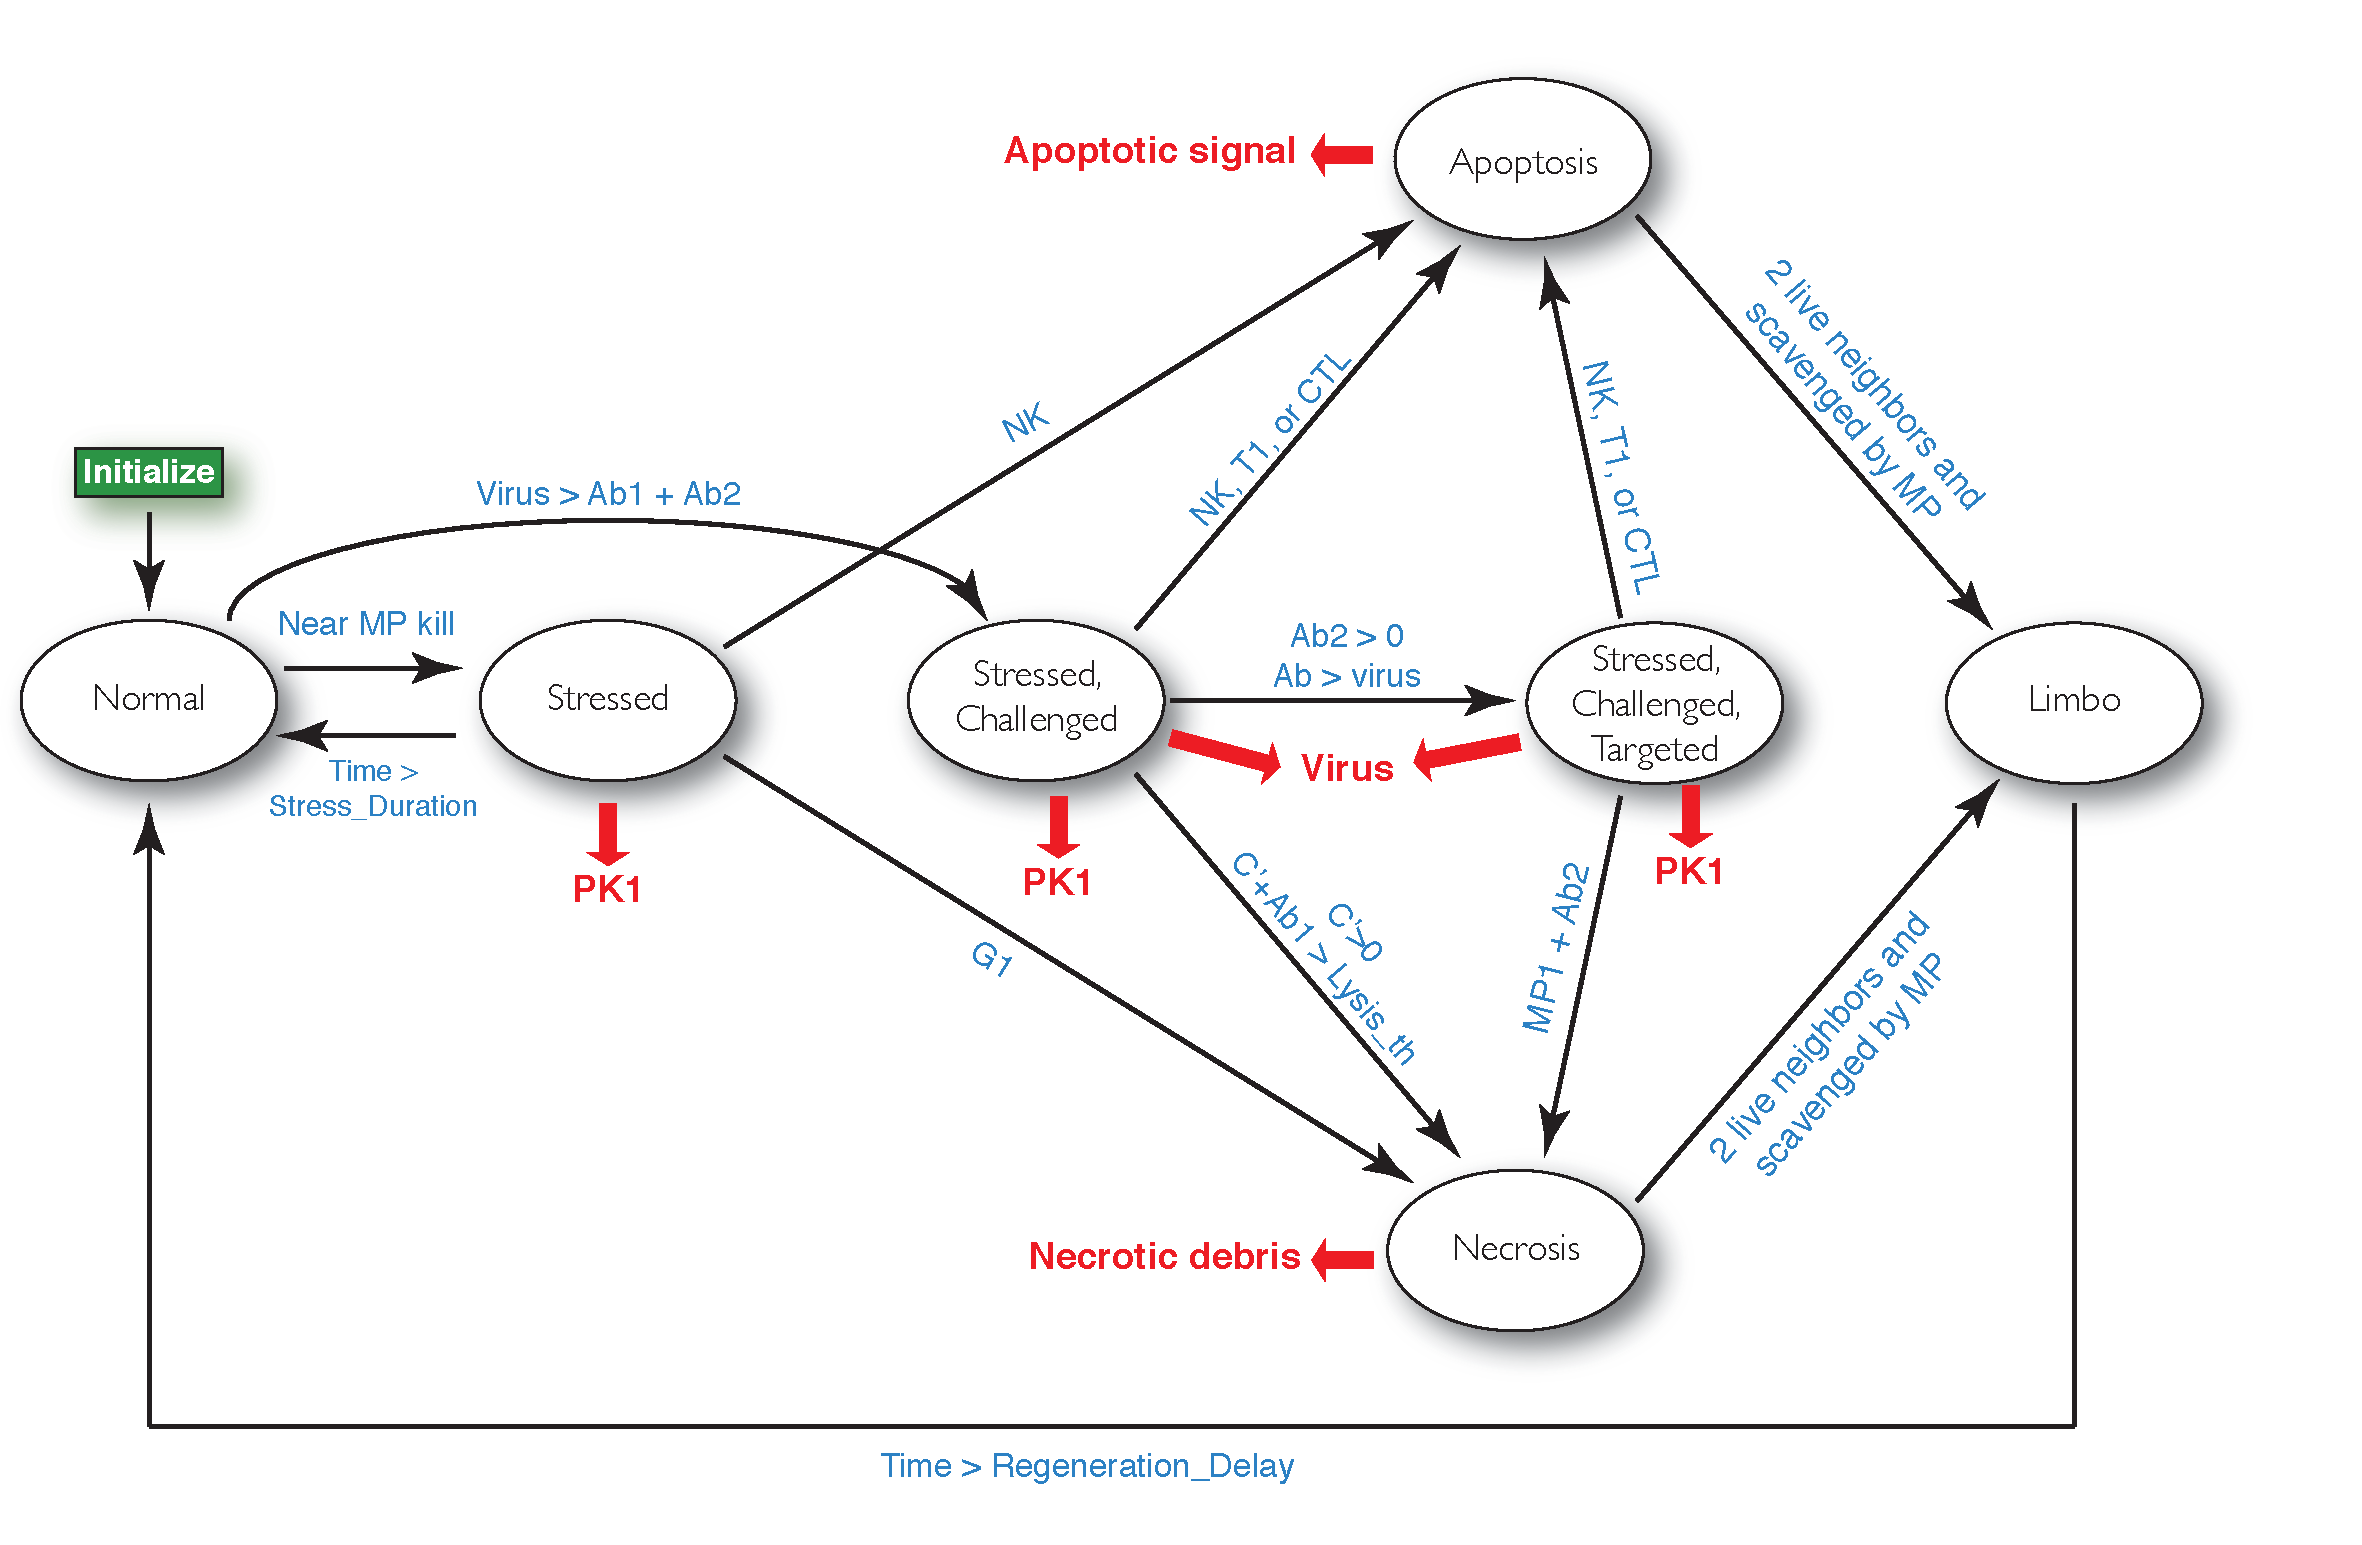
\includegraphics[width=7in]{PC_fsm}
% \includegraphics[width=\textwidth]{Parenchymal_Cell_State_Machine}
\caption{Parenchymal Cell state machine. Shows the state transition rules for
    the PC\@. As shown, the PC can either be Stressed: it detects virus signal,
    Challenged (infected), Apoptotic: it's been killed by an NK cell, Necrotic:
    it's been killed by a macrophage, or in Limbo: it's waiting to regenerate
    for a specified number of ticks.}
\label{PC_fsm}
\end{figure*}
% \end{figure*}

Cells, modeled as agents in the updated BIS, model both functional tissue and
the cells of the innate immune system. Cells can probe their Moore neighborhood
-- the 8 cells in their immediate vicinity and the one they are in -- and
detect agents and cells within it. Cells that can move begin by moving randomly
before discovering signals whose gradients they are programmed to follow.

\indent
Parenchymal Cells represent functional tissue. These cells get infected and
release stress and virus signals, spreading the infection and signaling their
own status. These cells cannot move and are typically surrounded by 4 other
cells of their own kind. They regenerate after a certain amount of time once
they have been scavenged by Macrophage cells. The updated BIS adds an infection
incubation period, during which the infected Parenchymal Cell releases no virus
signal. Upon conclusion of this period, the Parenchymal Cell releases a burst
of virus signal. The behavior of Parenchymal Cells is detailed in
Figure~\ref{PC_fsm}.

\indent
The updated BIS uses Macrophages and Natural Killer cells to model the activity
of the innate immune system. Macrophages perform dual function: infected cell
destruction and scavenging. These cells follow chemical gradients of PC signal
emissions in order to find infected, apoptotic, and necrotic PC cells, killing
or scavenging them. Natural Killer cells can only kill PC cells, also following
the chemical gradients of PC cells' various signals.

\indent
Certain agents possess input parameters that determine their lifespan. These
parameters are, in some cases, modified by specific state transition.

\subsection{Simulation Zones}
The original BIS used three "zones" of cell activity to represent different
areas in the body where cell interactions occur. These three zones represented
functional tissue, the lymph nodes, and the circulatory system
respectively~\cite{Folcik:2007}. In the updated BIS, there is only one zone and
it represents the generic functional tissue. This zone uses the same geometric
configuration as the zones in the original BIS do, a square two-dimensional
torus. The updated BIS zone has dimensions of 30x30. The zone used represents a
small slice of tissue, only large enough to allow the virus to take hold and
spread. Exact zone size was selected so as to allow the simulation to run for a
reasonable (more than 100 ticks) length in a reasonable amount of time (under
one minute).

\indent
Unfortunately, since the number of immune cells that react to pathogens is both
unknown and not easily translatable to this model, initial cell counts were
selected in order to produce the desired simulation response. Agents are
released from storage cells, called Portals, when the portals detect PC stress
signal (PK1) in the single cell that they monitor. This behavior simulates the
movement of innate immune cells in to stressed functional tissue in the body in
response to a foreign pathogen.

\subsection{Signal Diffusion and Time}
The updated BIS uses the same model of "ticks" and signal diffusion as the
original BIS~\cite{Folcik:2007}. Signals diffuse into the surrounding
environment fairly rapidly as a result.


\noindent

\section{Results}
\noindent
result

\section{Discussion}
\noindent
discuss

\bibliographystyle{IEEEtran_etalRoman}
\bibliography{refs.bib}

\end{document}
